\documentclass{article}
\usepackage[utf8]{inputenc}
\usepackage[spanish]{babel}
\usepackage{amsthm}
\usepackage{amssymb}
\usepackage{amsmath}
\usepackage{fancyhdr}
\usepackage{graphicx}
\usepackage[dvipsnames, table]{xcolor}
\usepackage[framemethod=tikz]{mdframed}
\usepackage{multicol}
\usepackage{tabularx}
\usepackage{pifont}
\setlength{\tabcolsep}{3pt}
\newcommand{\xmark}{\ding{55}}
\definecolor{mycolor}{rgb}{0.122, 0.435, 0.698}

\newmdenv[innerlinewidth=0.5pt, roundcorner=4pt,linecolor=mycolor,innerleftmargin=6pt,
innerrightmargin=6pt,innertopmargin=6pt,innerbottommargin=6pt]{mybox}

\newtheorem{definition}{Definición}
\newtheorem{proposition}{Proposición}



\setlength\parindent{0pt}

\renewcommand{\headrulewidth}{0.4pt}

\begin{document}
\date{6 - 13 de marzo de 2020}
\title{ \textbf{Topología} \\
Semana 1: Espacios topológicos y bases para topologías}
%\author{Docente: Gabriel Chicas Reyes, MSc.\\ 
	%			Alumno: Kevin López Aquino }
\maketitle	
\begin{mybox}
	\textbf{1. }  Sea $X$ un espacio topológico y $A$ un subconjunto de $X$. Supongamos que para cada $x \in A$ existe un conjunto abierto $U$ que contiene a $x$ tal que $U \subseteq A$. Demuestre que $U$ es abierto. 
\end{mybox}	

\begin{proof}
	Sea $\mathcal{U}$ la colección de todos los abiertos contenidos en $A$. Entonces, podemos escribir que
	$A =  \bigcup \mathcal{U} . $ Al ser $\mathcal{U}$ una colección de abiertos, $\bigcup \mathcal{U}$ también es un abierto. Por tanto, $A$ es abierto. 
\end{proof}

\begin{mybox}
	\textbf{2. }Considere las nueve topologías sobre $X = \{ a, b, c\}$  indicadas en la siguiente imagen y compárelas.  
\end{mybox}	

\begin{figure}[h]
\centering 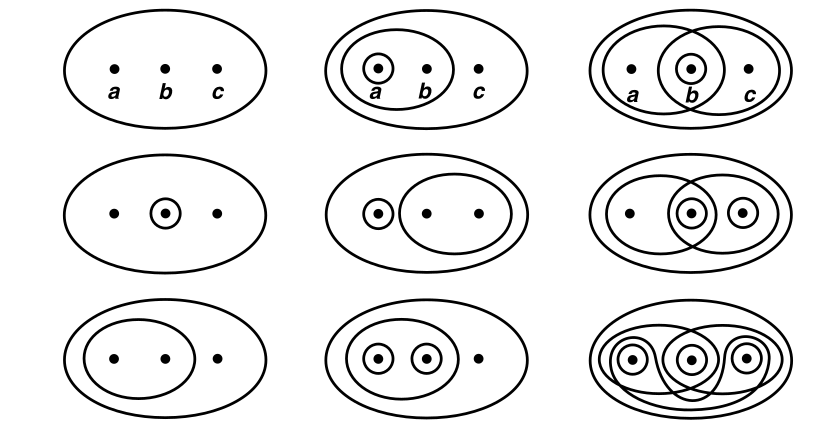
\includegraphics{fig1.png}
\caption{Nueve topologías sobre $X = \{a, b, c\}$. Tomado de §12 de \textbf{[1]}. }
\end{figure}
Numeramos las topologías de arriba abajo y de izquierda a derecha. Presentamos los resultados en la siguiente tabla, donde todas las inclusiones son estrictas y  el símbolo \textcolor{red}{\xmark} denota que las topologías no son comparables.
\begin{table}[h]
	\begin{tabularx}{\textwidth}{|X|X|c|c|c|c|c|c|c|c|}
		\hline
		  &$\mathcal{T}_{1}$   &$\mathcal{T}_{2}$ & $\mathcal{T}_{3}$ & $\mathcal{T}_{4}$ &  $\mathcal{T}_{5}$ &  $\mathcal{T}_{6}$ &$\mathcal{T}_{7}$ &  $\mathcal{T}_{8}$ & $\mathcal{T}_{9}$ \\ \hline
		 $\mathcal{T}_{1}$ &\cellcolor{green!25}  & $\mathcal{T}_{1} \subseteq \mathcal{T}_{2}$ & $\mathcal{T}_{1} \subseteq \mathcal{T}_{3}$ & $\mathcal{T}_{1} \subseteq \mathcal{T}_{4}$ & $\mathcal{T}_{1} \subseteq \mathcal{T}_{5}$ & $\mathcal{T}_{1} \subseteq \mathcal{T}_{6}$ &  $\mathcal{T}_{1} \subseteq \mathcal{T}_{7}$ & $\mathcal{T}_{1} \subseteq \mathcal{T}_{8}$ & $\mathcal{T}_{1} \subseteq \mathcal{T}_{9}$  \\ \hline
		 
		 $\mathcal{T}_{2}$ &  & \cellcolor{green!25} & \textcolor{red}{\xmark} & \textcolor{red}{\xmark} & \textcolor{red}{\xmark} & \textcolor{red}{\xmark} & $\mathcal{T}_{7} \subseteq \mathcal{T}_{2}$  & 
		 $\mathcal{T}_{2} \subseteq \mathcal{T}_{8}$ & $\mathcal{T}_{2} \subseteq \mathcal{T}_{9}$  \\ \hline
		 
		 $\mathcal{T}_{3}$ &  &  & \cellcolor{green!25} & $\mathcal{T}_{4} \subseteq \mathcal{T}_{3}$ & \textcolor{red}{\xmark} & $\mathcal{T}_{3} \subseteq \mathcal{T}_{6}$ &  $\mathcal{T}_{7} \subseteq \mathcal{T}_{3}$& \textcolor{red}{\xmark} & $\mathcal{T}_{3} \subseteq \mathcal{T}_{9}$ \\ \hline
		 
		 $\mathcal{T}_{4}$ &  &  &  & \cellcolor{green!25} & \textcolor{red}{\xmark} & $\mathcal{T}_{4} \subseteq \mathcal{T}_{6}$ &  \textcolor{red}{\xmark} & $\mathcal{T}_{4} \subseteq \mathcal{T}_{8}$  & $\mathcal{T}_{4} \subseteq \mathcal{T}_{9}$ \\ \hline
	    
	    $\mathcal{T}_{5}$ &  &  &  &  & \cellcolor{green!25} & \textcolor{red}{\xmark} &  \textcolor{red}{\xmark} & \textcolor{red}{\xmark}  & $\mathcal{T}_{5} \subseteq \mathcal{T}_{9}$ \\ \hline
	
	 $\mathcal{T}_{6}$ &  &  &  &  &  & \cellcolor{green!25} &  $\mathcal{T}_{7} \subseteq \mathcal{T}_{6}$ & \textcolor{red}{\xmark} & $\mathcal{T}_{6} \subseteq \mathcal{T}_{9}$  \\ \hline
		
		 $\mathcal{T}_{7}$ &  &  &  &  &  &  &  \cellcolor{green!25} & $\mathcal{T}_{7} \subseteq \mathcal{T}_{8}$ & $\mathcal{T}_{7} \subseteq \mathcal{T}_{9}$ \\ \hline
		
		 $\mathcal{T}_{8}$ &  &  &  &  &  &  &   & \cellcolor{green!25} & $\mathcal{T}_{8} \subseteq \mathcal{T}_{9}$  \\ \hline
		
		$\mathcal{T}_{9}$ &  &  &  &  &  &  &   &   & \cellcolor{green!25} \\ \hline
	\end{tabularx}
\end{table}

\begin{mybox}
	\textbf{3. (a)} Sea $X$ un conjunto y definamos 
	$$ \mathcal{T}_{c} =\{ U \subseteq X \mid U \text{ es conumerable en }X \} \cup \{\varnothing \}. $$
	Demuestre que $\mathcal{T}_{c}$ es una topología sobre $X$. \\

	\textbf{(b)} Considere la colección 
	$$ \mathcal{T}_{\infty} = \{ U \subseteq X \mid X \backslash U \text{ es infinito } \} \cup \{ \varnothing, X \}. $$
¿Es una topología sobe $X$?
\end{mybox}	

\begin{proof}
	Notamos que $\varnothing$ y $X$ están en $\mathcal{T}_{c}$. El primero por definición y el segundo por ser conumerable. \\
	Ahora supongamos que $\{ U_{\alpha}\}_{\alpha \in J}$ es una colección de conjuntos de $\mathcal{T}_{c}$ y demostremos que la unión de estos conjuntos también está en $\mathcal{T}_{c}$. Si la colección es vacía, este hecho se cumple dado que obtenemos el conjunto vacío. Si no, consideremos la expresión
	$$ X \backslash \bigcup_{\alpha \in J} U_{\alpha} = \bigcap_{\alpha \in J} (X \backslash U_{\alpha}). $$ 
	Si algún $U_{\alpha}$ es vacío, podemos descartarlo en el lado izquierdo, ya que no afecta a la unión. Así, si suponemos que $U_{\alpha} \neq \varnothing$ , se sigue que cada conjunto $X \backslash U_{\alpha}$ es finito, de forma que la expresión del lado derecho es la intersección de conjuntos finitos y debe ser, por tanto, finita. Esto implica que $\bigcup_{\alpha \in J} U_{\alpha}$ está en $\mathcal{T}_{\alpha}$.\\
	Sean $U_{1}, U_{2}$ elementos de $\mathcal{T}_{c}$ y supongamos que ninguno es vacío. Entonces,
	$$ X \backslash (U_{1} \cap U_{2}) = (X \backslash U_{1}) \cup (X \backslash U_{2}) $$
	es un conjunto finito, dado que es la unión de dos conjuntos finitos. Por tanto, $U_{1} \cap U_{2}$ está en $\mathcal{T}_{c}$.
\end{proof} 
\textbf{Comentario. } De la definición notamos que si $X$ es un conjunto numerable, $\mathcal{T}_{c}$ coincide con la topología discreta sobre $X$.\\

Para \textbf{(b)} notamos que si $X$ es finito, $\mathcal{T}_{\infty} = \{ \varnothing, X \}$. Por el contrario, si $X$ es infinito, $\mathcal{T}_{\infty}$ no es una topología. Consideremos un contraejemplo en $\mathbb{R}$. Los conjuntos $(-\infty, 1)$ y $(1, \infty )$ están en $\mathcal{T}_{\infty}$, pero su unión no, dado que $\mathbb{R} \backslash ( (- \infty, 1) \cup (1, \infty) ) = \{ 1 \}$. \hspace{7cm} $\blacksquare$
\vspace{0.5cm}

\begin{mybox}
	\textbf{4. (a)} Si $\{ \mathcal{T_{\alpha}} \}$ es una familia de topologías sobre $X$, demuestre que $\bigcap \mathcal{T_{\alpha}}$ es una topología sobre $X$.  ¿Es $\bigcup \mathcal{T}_{\alpha}$ una topología sobre $X$? \\
	
	\textbf{(b)} Demuestre que existe una única topología más grande contenida en todas las topologías $\{\mathcal{T}_{\alpha} \}$ y que existe una única topología más pequeña que contiene a todas estas topologías. \\
	
	\textbf{(c)} Si $X = \{a, b, c \}$, sean 
	$$ \mathcal{T}_{1} = \{ \varnothing, X, \{a \}, \{a, b \} \} \text{ y } \mathcal{T}_{2} = \{ \varnothing, X, \{a \}, \{b, c \} \}.$$
	Encuentre la topología más pequeña que contiene a $\mathcal{T}_{1}$ y $\mathcal{T}_{2}$ y la topología más grande contenida en $\mathcal{T}_{1}$ y $\mathcal{T}_{2}$.
\end{mybox}	

$ \textbf{(a)}$ Sea $\{ \mathcal{T_{\alpha}}\}$ una familia de topologías sobre un conjunto $X$. Al estar en cada topología $\mathcal{T_{\alpha}}$, los conjuntos $X$ y $\varnothing$ también están en $\bigcap \mathcal{T_{\alpha}}$. \\
Si $\{U_{\beta} \}$ es una subcolección de $ \bigcap \mathcal{T}_{\alpha}$, se sigue que cada uno de los conjuntos $U_{\beta}$ es un abierto en cada topología $\mathcal{T_{\alpha}}$. Así, $\bigcup U_{\beta}$ también es un abierto en cada $\mathcal{T}_{\alpha}$, de lo que se sigue que $\bigcup U_{\beta} \in \bigcap \mathcal{T}_{\alpha}.$ \\
Ahora supongamos que $U_{1}$ y $U_{2}$ están en $\bigcap \mathcal{T_{\alpha}}$. Se sigue que estos dos conjuntos son abiertos en cada topología $\mathcal{T}_{\alpha}$, por lo que su intersección también es abierta en cada topología $\mathcal{T}_{\alpha}$. Así, $U_{1} \cap U_{2} \in \bigcap \mathcal{T_{\alpha}}$. \\

En contraste, la unión de topologías no es necesariamente una topología. Consideremos el conjunto $X = \{ a, b, c\}$ y las topologías
$$ \mathcal{T}_{1} = \{ \varnothing, X, \{ b \}  \} \text{ y  } \mathcal{T}_{2} = \{ \varnothing, X, \{ a \}, \{ b, c \}  \} .$$
Entonces, $\mathcal{T}_{1} \cup \mathcal{T}_{2} = \{ \varnothing, X, \{ a \}, \{ b \}, \{ b, c \} \}$, pero $\{ a \} \cup \{ b \} \notin \mathcal{T}_{1} \cup \mathcal{T}_{2}$. $\hspace*{\fill} \blacksquare$\\

\textbf{(b) } Para ver que existe una única topología más grande contenida en todas las topologías $\mathcal{T}_{\alpha}$ notamos que $\bigcap \mathcal{T}_{\alpha}$ es una topología. Esta topología está contenida en todas las topologías $\mathcal{T}_{\alpha}$. Si $\mathcal{T}$ es una topología que cumple con esta propiedad, se deduce que $\mathcal{T} \subseteq \bigcap \mathcal{T}_{\alpha} $, de forma que esta última es la topología más grande que cumple con esta propiedad.  \\

Para demostrar que existe una única topología más pequeña que contiene a todas las topologías $\mathcal{T}_{\alpha}$, notamos que si bien no podemos esperar que $\bigcup \mathcal{T}_{\alpha}$ sea una topología, sí es una subbase. Por el \textbf{ejercicio 5}, la topología generada por esta subbase es la topología más pequeña que contiene a los elementos de la subbase como elementos. $\hspace*{\fill} \blacksquare$\\

\textbf{(c)} La topología más grande que está contenida en $\mathcal{T}_{1}$ y $\mathcal{T}_{2}$ es
$$ \bigcap \{ \mathcal{T}_{1}, \mathcal{T}_{2} \}  =  \mathcal{T}_{1} \cap \mathcal{T}_{2} = \{ \varnothing, X,  \{a \} \}.$$
Para encontrar la topología más pequeña que contiene a $\mathcal{T}_{1}$ y $\mathcal{T}_{2}$, primero calculamos $\bigcup \{\mathcal{T}_{1}, \mathcal{T}_{2} \}$:
$$ \bigcup \{\mathcal{T}_{1}, \mathcal{T}_{2} \} = \mathcal{T}_{1} \cup \mathcal{T}_{2} = \{ \varnothing, X, \{a, b \}, \{b, c \},\{a \} \}.$$
Ahora calculamos el conjunto de todas las intersecciones finitas de elementos de la subbase:
$$\mathcal{B} = \{ \varnothing, X, \{a, b \}, \{b, c \},\{a \}, \{b \} \}.$$
Para obtener la topología deseada, tomamos uniones arbitrarias de elementos de $\mathcal{B}$. En este caso, resulta que la topología es igual a $\mathcal{B}$. $\hspace*{\fill} \blacksquare$\\
\vspace{0.5cm}
\begin{mybox}
	\textbf{5. } Demuestre que si $\mathcal{A}$ es una base para una topología sobre $X$, entonces la topología generada por $\mathcal{A}$ es igual a la intersección de todas las topologías sobre $X$ que contienen a $\mathcal{A}.$ Pruebe lo mismo para una subbase. 
\end{mybox}	

 \textbf{Comentario. } Los siguientes resultados nos dicen que si $\mathcal{B}$ es una base, la topología generada por $\mathcal{B}$ es la topología más pequeña que contiene que $\mathcal{B}$. De forma análoga, si $\mathcal{S}$ es una subbase, la topología que genera es la topología más pequeña de entre todas las topologías que contienen a $\mathcal{S}$. \\

$\bullet$ Supongamos que $\mathcal{A}$ es una base que genera una topología $\mathcal{T_{A}}$ y sea
$$ \mathrm{T} = \{ \mathcal{T} \mid \mathcal{T} \text{ es una topología sobre }X \text{ y }\mathcal{A}\subseteq \mathcal{T} \} .$$
Notamos que $\mathcal{T_{A}} \in \mathrm{T}$, de forma que $\bigcap \mathrm{T} \subseteq \mathcal{T_{A}}$.\\
Por otro lado,  si $U$ es un abierto de la topología generada por $\mathcal{A}$, podemos escribir
$$ U = \bigcup_{\alpha \in J} A_{\alpha} $$
donde $\{A_{\alpha} \}_{\alpha \in J}$ son elementos de $\mathcal{A}$. Cada $A_{\alpha}$ pertence a cada topología en $\mathrm{T}$, de lo que se sigue que su unión también debe pertencer a cada topología contenida en $\mathrm{T}.$ Así,  $\mathcal{T_{A}} \subseteq \bigcap \mathrm{T}. \hspace*{\fill} \blacksquare$\\

$\bullet $ Ahora supongamos que $\mathcal{S}$ es una subbase y sea
$$  \mathrm{T} = \{ \mathcal{T} \mid \mathcal{T} \text{ es una topología sobre }X \text{ y }\mathcal{S}\subseteq \mathcal{T} \} .$$
 Notamos que la topología $\mathcal{T}_{\mathcal{S}}$ está $\mathrm{T}$, de lo que podemos deducir que $\bigcap \mathrm{T} \subseteq \mathcal{T_{S}}$. Si $U$ es un abierto de $\mathcal{T_{S}}$, es la unión de intersecciones finitas de elementos de $\mathcal{S}$. Puesto que los elementos de $\mathcal{S}$ están en cada topología de $\mathrm{T}$, sus intersecciones finitas también estarán en cada topología, al igual que cualquier unión de estas. Por tanto, $\mathcal{T_{S}} \subseteq \bigcap \mathrm{T}$. $\hspace*{\fill} \blacksquare$\\ 
\begin{mybox}
\textbf{6. } Demuestre que las topologías de $\mathbb{R}_{\ell}$ y de $\mathbb{R}_{K}$ no son comparables. 	
\end{mybox}	

$\bullet$  Supongamos que el abierto $[0, 1)$ de la topología de $\mathbb{R}_{\ell}$ es abierto en la topología de $\mathbb{R}_{K}$. Entonces, debe existir un conjunto ya sea de la forma $(a, b)$ o de la forma $(a, b) \backslash K$ que contenga a $0$ y esté contenido en $[0, 1)$ pero ninguno de estos casos es posible. $\hspace*{\fill} \blacksquare$\\

$\bullet$ El conjunto $(-1, 1) \backslash K$ es abierto en la topología de $\mathbb{R}_{K}$, pero no puede ser abierto en la topología de $\mathbb{R}_{\ell}$, ya que existiría algún $[a, b)$ tal que
$$ 0 \in [a, b) \subseteq (-1, 1)\backslash K $$
y cualquier $[a, b)$ contendría elementos de $K$. $\hspace*{\fill} \blacksquare$\\

\begin{mybox}
	\textbf{7. } Considere las siguientes topologías sobre $\mathbb{R}:$ \\
	
	$ \mathcal{T}_{1} = $ la topología usual, \\
	$\mathcal{T}_{2} = $ la topología de $\mathbb{R}_{K}$, \\
	$\mathcal{T}_{3} = $ la topología cofinita, \\
	$\mathcal{T}_{4} = $ la topología del límite superior, con todos los conjuntos $(a, b ]$ como base, \\
	$\mathcal{T}_{5} = $ la topología con todos los conjuntos $(- \infty, a)$ como base.  \\
	
	Determine las posibles relaciones de inclusión entre estas topologías. 
\end{mybox}	
 \begin{table}[h]
 	\begin{tabularx}{\textwidth}{|X|X|X|X|X|X|}
 		\hline
 		&$\mathcal{T}_{1}$   &$\mathcal{T}_{2}$ & $\mathcal{T}_{3}$ & $\mathcal{T}_{4}$ & $\mathcal{T}_{5}$ \\ \hline
 		
 		$\mathcal{T}_{1}$ &  \cellcolor{blue!25} &(1) $\mathcal{T}_{1} \subseteq \mathcal{T}_{2}$ &(2) $\mathcal{T}_{3} \subseteq \mathcal{T}_{1}$  &(3) $\mathcal{T}_{1} \subseteq \mathcal{T}_{4}$ &(4) $\mathcal{T}_{5} \subseteq \mathcal{T}_{1}$ \\ \hline
 		
 		$\mathcal{T}_{2}$ &  &  \cellcolor{blue!25} &(5) $\mathcal{T}_{3} \subseteq \mathcal{T}_{2}$  &(6) \hspace{0.2cm} \textcolor{red}{\xmark} &(7) $\mathcal{T}_{5} \subseteq \mathcal{T}_{2}$ \\ \hline
 		
 		$\mathcal{T}_{3}$ &  &  & \cellcolor{blue!25} &(8) $\mathcal{T}_{3} \subseteq \mathcal{T}_{4}$ &(9) \hspace{0.2cm} \textcolor{red}{\xmark} \\ \hline
 		
 		$\mathcal{T}_{4}$ &  &  &  & \cellcolor{blue!25} &(10)$\mathcal{T}_{5} \subseteq \mathcal{T}_{4}$ \\ \hline
 		
 		$\mathcal{T}_{5}$ &  &  &  &  & \cellcolor{blue!25} \\ \hline
 		
 		\end{tabularx}
 \end{table}
\newpage
$\textbf{(1)}$ La topología de $\mathbb{R}_{K}$ es estrictamente más fina que la topología usual. \\

$\textbf{(2)}$ Sea $U$ un abierto de la topología cofinita. Entonces, $U$ contiene a todos los números reales salvo una cantidad finita de estos.  Supongamos que 
$$ x_{0} < x_{1} < \ldots < x_{n-1} < x_{n} $$
son los números reales que no están en $U$. Podemos escribir
$$ U = (-\infty, x_{0}) \cup (x_{0}, x_{1}) \cup \ldots \cup (x_{n-1}, x_{n}) \cup (x_{n}, \infty). $$
Notamos que 
$$ (-\infty, x_{0}) = \bigcup \{ (r, x_{0}) \subseteq \mathbb{R} \mid r < x_{0} \} $$
$$(x_{n},\infty) = \bigcup \{ (x_{n}, r) \subseteq \mathbb{R} \mid x_{n} < r  \}, $$
de forma que cada abierto de $\mathcal{T}_{c}$ se puede expresar como la unión de intervalos abiertos. La inclusión es estricta: los intervalos $(a, b)$ no son cofinitos. \\

$\textbf{(3)}$ La topología usual es estrictamente más gruesa que la topología del límite superior. Dado un intervalo $(a, b)$, para todo $x \in (a, b)$ tenemos que $x \in (a, x] \subseteq (a, b)$. Para ver que la inclusión es estricta, se debe notar que todos los conjuntos de la forma $(a, b]$ son abiertos en la topología del límite superior, pero no pueden serlo en la topología usual, ya que no hay forma de encontrar un intervalo abierto que incluya a $b$ y esté contenido en $(a, b]$. \\

$\textbf{(4)}$ Para cada $x \in (-\infty, a)$ podemos encontrar un intervalo abierto que contenga a $x$ y esté dentro de $(-\infty, a)$. La inclusión es estricta: ningún intervalo $(a, b)$ puede pertenecer a la topología $\mathcal{T}_{5}$. \\

$\textbf{(5)}$ Al ser estrictamente más gruesa que la topología usual, se sigue que la topología cofinita es estrictamente más gruesa que la topología de $\mathbb{R}_{K}$.\\

$\textbf{(6)}$ Las topologías de $\mathbb{R}_{K}$ y del límite superior no son comparables. Un argumento análogo al del \textbf{ejercicio 6} se puede hacer para probar esto, sustituyendo los conjuntos de la forma $[a,b)$ por conjuntos de la forma $(a,b]$. \\

$\textbf{(7)}$ $\mathcal{T}_{5}$ es estrictamente más gruesa que la topología usual, de forma que también debe ser estrictamente más gruesa que la topología de $\mathbb{R}_{K}$. \\

$\textbf{(8)}$ La topología cofinita es estrictamente más gruesa que la topología usual y esta es estrictamente más gruesa que la topología del límite superior como se demostró en $\textbf{(2)}$.\\ 
\newpage
$\textbf{(9)}$ La topología cofinita y $\mathcal{T}_{5}$ no son comparables. Por un lado, los conjuntos de la forma $(- \infty, a)$ no son cofinitos. Por otro lado, el conjunto $\mathbb{R} \backslash \{ 1, 2\}$ está en $\mathcal{T}_{3}$, pero no hay forma que esté en $\mathcal{T}_{5}: $ de lo contrario, existiría un conjunto $(-\infty, a)$ tal que
$$  2 \in (\infty, a) \subseteq \mathbb{R} \backslash \{1, 2 \}.$$ 
Entonces, $1 \in (- \infty, a)$, aun cuando lo hemos removido del conjunto de la derecha. \\

$\textbf{(10)}$ La topología $\mathcal{T}_{5}$ es estrictamente más gruesa que la topología usual y esta es estrictamente más gruesa que la topología del límite superior, de forma que $\mathcal{T}_{5}$ es estrictamente más gruesa que la topología del límite superior. $\hspace*{\fill} \blacksquare$\\
 

\begin{mybox}
\textbf{8. (a)} Aplique el \textbf{lema 13.2} para demostrar que la colección contable 
$$ \mathcal{B} = \{ (p, q) \subseteq \mathbb{R} \mid p < q \text{ y } p, q \in \mathbb{Q} \} $$
es una base que genera la topología estándar sobre $\mathbb{R}$.	\\

\textbf{(b) }Demuestre que la colección 
$$ \mathcal{C} = \{ [p, q) \subseteq \mathbb{R} \mid p < q \text{ y }p, q \in \mathbb{Q} \} $$
es una base que genera una topología diferente de la topología del límite inferior sobre $\mathbb{R}$.
\end{mybox}	

\textbf{(a)} Consideremos un abierto $U$ en la topología estándar y un elemento $x$ de este. Entonces, existen $a, b \in \mathbb{R}$ tales que $x \in (a, b) \subseteq U$. Podemos elegir racionales $p, q$ tales que 
$$ a < p < x < q < b ,$$
de modo que $x \in (p, q) \subseteq (a, b ) \subseteq U.$ Se sigue que $\mathcal{B}$ es una base que genera la topología estándar sobre $\mathbb{R}$. $\hspace*{\fill} \blacksquare$\\

\textbf{(b) } Notemos que $[\sqrt{2}, \frac{3}{2})$ es abierto en la topología de $\mathbb{R}_{\ell}$. Procedemos por contradicción. Supongamos que $[\sqrt{2}, \frac{3}{2})$ es abierto en la topología generada por $\mathcal{C}$. Entonces, existen racionales $p$ y $q$ tales que $\sqrt{2} \in [p, q) \subseteq [\sqrt{2}, \frac{3}{2})$. Esto implica que $p < \sqrt{2}$ y $p > \sqrt{2}$, de lo que deducimos que $[\sqrt{2}, \frac{3}{2})$ no puede pertenecer a la topología generada por $\mathcal{C}$. \\
Por otro lado, se cumple que la topología generada por $\mathcal{C}$ es más gruesa que la topología de $\mathbb{R}_{\ell}$, ya que todos los elementos de $\mathcal{C}$ están en la base que genera la topología de $\mathbb{R}_{\ell}$. $\hspace*{\fill} \blacksquare$
\section*{Referencia}
\textbf{[1]} Munkres, J. R. (2014). \textit{Topology}, segunda edición internacional. Pearson Education. 

\end{document}
